%% abtex2-modelo-trabalho-academico.tex, v-1.9.7 laurocesar
%% Copyright 2012-2018 by abnTeX2 group at http://www.abntex.net.br/ 
%%
%% This work may be distributed and/or modified under the
%% conditions of the LaTeX Project Public License, either version 1.3
%% of this license or (at your option) any later version.
%% The latest version of this license is in
%%   http://www.latex-project.org/lppl.txt
%% and version 1.3 or later is part of all distributions of LaTeX
%% version 2005/12/01 or later.
%%
%% This work has the LPPL maintenance status `maintained'.
%% 
%% The Current Maintainer of this work is the abnTeX2 team, led
%% by Lauro César Araujo. Further information are available on 
%% http://www.abntex.net.br/
%%
%% This work consists of the files abntex2-modelo-trabalho-academico.tex,
%% abntex2-modelo-include-comandos and abntex2-modelo-references.bib
%%

% ------------------------------------------------------------------------
% ------------------------------------------------------------------------
% abnTeX2: Modelo de Trabalho Academico (tese de doutorado, dissertacao de
% mestrado e trabalhos monograficos em geral) em conformidade com 
% ABNT NBR 14724:2011: Informacao e documentacao - Trabalhos academicos -
% Apresentacao
% ------------------------------------------------------------------------
% ------------------------------------------------------------------------

\documentclass[
	% -- opções da classe memoir --
	12pt,				% tamanho da fonte
	openright,			% capítulos começam em pág ímpar (insere página vazia caso preciso)
	twoside,			% para impressão em recto e verso. Oposto a oneside
	a4paper,			% tamanho do papel. 
	% -- opções da classe abntex2 --
	%chapter=TITLE,		% títulos de capítulos convertidos em letras maiúsculas
	%section=TITLE,		% títulos de seções convertidos em letras maiúsculas
	%subsection=TITLE,	% títulos de subseções convertidos em letras maiúsculas
	%subsubsection=TITLE,% títulos de subsubseções convertidos em letras maiúsculas
	% -- opções do pacote babel --
	english,			% idioma adicional para hifenização
	brazil				% o último idioma é o principal do documento
	]{abntex2}

% ---
% Pacotes básicos 
% ---
\usepackage{lmodern}			% Usa a fonte Latin Modern			
\usepackage[T1]{fontenc}		% Selecao de codigos de fonte.
\usepackage[utf8]{inputenc}		% Codificacao do documento (conversão automática dos acentos)
\usepackage{indentfirst}		% Indenta o primeiro parágrafo de cada seção.
\usepackage{color}				% Controle das cores
\usepackage{graphicx}			% Inclusão de gráficos
\usepackage{microtype} 			% para melhorias de justificação
\usepackage{adjustbox}          % Quadros justificados
\usepackage{listings}
\usepackage{xcolor}

% ---
		
% ---
% Pacotes adicionais, usados apenas no âmbito do Modelo Canônico do abnteX2
% ---
\usepackage{lipsum}				% para geração de dummy text
% ---

% ---
% Pacotes de citações
% ---
\usepackage[brazilian,hyperpageref]{backref}	 % Paginas com as citações na bibl
\usepackage[alf]{abntex2cite}	% Citações padrão ABNT

% --- 
% CONFIGURAÇÕES DE PACOTES
% --- 

% ---
% Configurações do pacote backref
% Usado sem a opção hyperpageref de backref
\renewcommand{\backrefpagesname}{Citado na(s) página(s):~}
% Texto padrão antes do número das páginas
\renewcommand{\backref}{}
% Define os textos da citação
\renewcommand*{\backrefalt}[4]{
	\ifcase #1 %
		Nenhuma citação no texto.%
	\or
		Citado na página #2.%
	\else
		Citado #1 vezes nas páginas #2.%
	\fi}%
% ---

\definecolor{codegreen}{rgb}{0,0.6,0}
\definecolor{codegray}{rgb}{0.5,0.5,0.5}
\definecolor{codepurple}{rgb}{0.58,0,0.82}
\definecolor{backcolour}{rgb}{0.95,0.95,0.92}

\lstdefinestyle{mystyle}{
    backgroundcolor=\color{backcolour},   
    commentstyle=\color{codegreen},
    keywordstyle=\color{magenta},
    numberstyle=\tiny\color{codegray},
    stringstyle=\color{codepurple},
    basicstyle=\ttfamily\footnotesize, % Ajuste aqui para o tamanho desejado
    breakatwhitespace=false,         
    breaklines=true,                 
    captionpos=b,                    
    keepspaces=true,                 
    numbers=left,                    
    numbersep=5pt,                  
    showspaces=false,                
    showstringspaces=false,
    showtabs=false,                  
    tabsize=2
}


\lstset{
    literate=%
        {á}{{\'a}}1 {é}{{\'e}}1 {í}{{\'i}}1 {ó}{{\'o}}1 {ú}{{\'u}}1
        {Á}{{\'A}}1 {É}{{\'E}}1 {Í}{{\'I}}1 {Ó}{{\'O}}1 {Ú}{{\'U}}1
        {à}{{\`a}}1 {è}{{\`e}}1 {ì}{{\`i}}1 {ò}{{\`o}}1 {ù}{{\`u}}1
        {À}{{\`A}}1 {È}{{\`E}}1 {Ì}{{\`I}}1 {Ò}{{\`O}}1 {Ù}{{\`U}}1
        {ã}{{\~a}}1 {õ}{{\~o}}1
        {Ã}{{\~A}}1 {Õ}{{\~O}}1
        {â}{{\^a}}1 {ê}{{\^e}}1 {î}{{\^i}}1 {ô}{{\^o}}1 {û}{{\^u}}1
        {Â}{{\^A}}1 {Ê}{{\^E}}1 {Î}{{\^I}}1 {Ô}{{\^O}}1 {Û}{{\^U}}1
        {ç}{{\c{c}}}1 {Ç}{{\c{C}}}1
        {ø}{{\o}}1 {å}{{\r a}}1
        {Ø}{{\O}}1 {Å}{{\r A}}1
}


\lstset{style=mystyle}

% ---
% Informações de dados para CAPA e FOLHA DE ROSTO
% ---
\titulo{PIM VIII \\ Projeto Integrado Multidiciplinar VIII}
\autor{Pedro Laurenti, Lucas Andrade e Allan Cândido}
\local{Brasil}
\data{Setembro de 2023}
\orientador{Robson Batista Alves}
\coorientador{Tarcisio Peres}
\instituicao{%
  Universidade Paulista - UNIP
  \par
  Curso de Análise e Desenvolvimento de Sistemas
  \par}
\tipotrabalho{Trabalho Científico}
% O preambulo deve conter o tipo do trabalho, o objetivo, 
% o nome da instituição e a área de concentração 
\preambulo{Trabalho científico redigido colocando em prática as habilidades e conhecimento adquiridos no terceiro período do curso.}
% ---


% ---
% Configurações de aparência do PDF final

% alterando o aspecto da cor azul
\definecolor{blue}{RGB}{41,5,195}

% informações do PDF
\makeatletter
\hypersetup{
     	%pagebackref=true,
		pdftitle={\@title}, 
		pdfauthor={\@author},
    	pdfsubject={\imprimirpreambulo},
	    pdfcreator={Pedro Laurenti, Lucas Andrade e Allan Cândido},
		pdfkeywords={Desenvolvimento}{Análise e Desenvolvimento}{Sistemas}{PIM VIII}{UNIP}, 
		colorlinks=true,       		% false: boxed links; true: colored links
    	linkcolor=blue,          	% color of internal links
    	citecolor=blue,        		% color of links to bibliography
    	filecolor=magenta,      		% color of file links
		urlcolor=blue,
		bookmarksdepth=4
}
\makeatother
% --- 

% ---
% Posiciona figuras e tabelas no topo da página quando adicionadas sozinhas
% em um página em branco. Ver https://github.com/abntex/abntex2/issues/170
\makeatletter
\setlength{\@fptop}{5pt} % Set distance from top of page to first float
\makeatother
% ---

% ---
% Possibilita criação de Quadros e Lista de quadros.
% Ver https://github.com/abntex/abntex2/issues/176
%
\newcommand{\quadroname}{Quadro}
\newcommand{\listofquadrosname}{Lista de quadros}

\newfloat[chapter]{quadro}{loq}{\quadroname}
\newlistof{listofquadros}{loq}{\listofquadrosname}
\newlistentry{quadro}{loq}{0}

% configurações para atender às regras da ABNT
\setfloatadjustment{quadro}{\centering}
\counterwithout{quadro}{chapter}
\renewcommand{\cftquadroname}{\quadroname\space} 
\renewcommand*{\cftquadroaftersnum}{\hfill--\hfill}

\setfloatlocations{quadro}{hbtp} % Ver https://github.com/abntex/abntex2/issues/176
% ---

% --- 
% Espaçamentos entre linhas e parágrafos 
% --- 

% O tamanho do parágrafo é dado por:
\setlength{\parindent}{1.3cm}

% Controle do espaçamento entre um parágrafo e outro:
\setlength{\parskip}{0.2cm}  % tente também \onelineskip

% ---
% compila o indice
% ---
\makeindex
% ---

% ----
% Início do documento
% ----
\begin{document}

% Seleciona o idioma do documento (conforme pacotes do babel)
%\selectlanguage{english}
\selectlanguage{brazil}

% Retira espaço extra obsoleto entre as frases.
\frenchspacing 

% ----------------------------------------------------------
% ELEMENTOS PRÉ-TEXTUAIS
% ----------------------------------------------------------
% \pretextual

% ---
% Capa
% ---
\imprimircapa
% ---

% ---
% Folha de rosto
% (o * indica que haverá a ficha bibliográfica)
% ---
\imprimirfolhaderosto*
% ---

% ---
% Inserir a ficha bibliografica
% ---

% Isto é um exemplo de Ficha Catalográfica, ou ``Dados internacionais de
% catalogação-na-publicação''. Você pode utilizar este modelo como referência. 
% Porém, provavelmente a biblioteca da sua universidade lhe fornecerá um PDF
% com a ficha catalográfica definitiva após a defesa do trabalho. Quando estiver
% com o documento, salve-o como PDF no diretório do seu projeto e substitua todo
% o conteúdo de implementação deste arquivo pelo comando abaixo:
%
% \begin{fichacatalografica}
%     \includepdf{fig_ficha_catalografica.pdf}
% \end{fichacatalografica}

\begin{fichacatalografica}
	\sffamily
	\vspace*{\fill}					% Posição vertical
	\begin{center}					% Minipage Centralizado
	\fbox{\begin{minipage}[c][8cm]{13.5cm}		% Largura
	\small
	\imprimirautor
	%Sobrenome, Nome do autor
	
	\hspace{0.5cm} PIM VIII Projeto Integrado Multidiciplinar VIII - 
	\imprimirlocal, \imprimirdata \ --
	
	\hspace{0.5cm} \thelastpage p.\\
	
	\hspace{0.5cm} \imprimirorientadorRotulo~\imprimirorientador\\
	
	\hspace{0.5cm}
	\parbox[t]{\textwidth}{\imprimirtipotrabalho~--~\imprimirinstituicao,
	\imprimirdata.}\\
	
	\hspace{0.5cm}
		1. Market Place.
		2. Desenvolvimento.
		3. Análise de Sistemas.
		I. Market.
		II. UNIP - Universidade Paulista.
		III. Faculdade de  Análise e Desenvolvimento de Sistemas.
		IV. PIM VIII - Projeto Integrado Multidiciplinar.  		
	\end{minipage}}
	\end{center}
\end{fichacatalografica}
% ---

% ---
% Inserir folha de aprovação
% ---

% Isto é um exemplo de Folha de aprovação, elemento obrigatório da NBR
% 14724/2011 (seção 4.2.1.3). Você pode utilizar este modelo até a aprovação
% do trabalho. Após isso, substitua todo o conteúdo deste arquivo por uma
% imagem da página assinada pela banca com o comando abaixo:
%
% \begin{folhadeaprovacao}
% \includepdf{folhadeaprovacao_final.pdf}
% \end{folhadeaprovacao}
%
\begin{folhadeaprovacao}

  \begin{center}
    {\ABNTEXchapterfont\large\imprimirautor}

    \vspace*{\fill}\vspace*{\fill}
    \begin{center}
      \ABNTEXchapterfont\bfseries\Large\imprimirtitulo
    \end{center}
    \vspace*{\fill}
    
    \hspace{.45\textwidth}
    \begin{minipage}{.5\textwidth}
        \imprimirpreambulo
    \end{minipage}%
    \vspace*{\fill}
   \end{center}
        
   Trabalho aprovado. \imprimirlocal, 24 de novembro de 2012:

   \assinatura{\textbf{\imprimirorientador} \\ Orientador} 
   \assinatura{\textbf{Professor} \\ Convidado 1}
   \assinatura{\textbf{Professor} \\ Convidado 2}
   %\assinatura{\textbf{Professor} \\ Convidado 3}
   %\assinatura{\textbf{Professor} \\ Convidado 4}
      
   \begin{center}
    \vspace*{0.5cm}
    {\large\imprimirlocal}
    \par
    {\large\imprimirdata}
    \vspace*{1cm}
  \end{center}
  
\end{folhadeaprovacao}
% ---

% ---
% Dedicatória
% ---
\begin{dedicatoria}
	\vspace*{\fill}
	\centering
	\noindent
	\textit{Este projeto é dedicado a todos os desenvolvedores que já falharam várias vezes, mas nunca desistiram de suas paixões e ideias.}
	\vspace*{\fill}

\end{dedicatoria}
% ---

% ---
% Agradecimentos
% ---
% \begin{agradecimentos}
% 	Os agradecimentos principais são direcionados à todos aqueles que contribuíram para que a produção deste trabalho acadêmico.
% 
% 	Agradecimentos especiais aos desenvolvedores do \abnTeX e ao professor Miguel Frasson - pelas orientações.
% 
% \end{agradecimentos}
% ---


% ---
% Epígrafe
% ---
\begin{epigrafe}
	\vspace*{\fill}
	\begin{flushright}
		\textit{``Ser feliz ao realizar a jornada pode ser muito melhor do que chegar ao destino com sucesso.'' - (Jordan Peterson)}
	\end{flushright}
\end{epigrafe}
% ---

% ---
% RESUMOS
% ---

% resumo em português
\setlength{\absparsep}{18pt} % ajusta o espaçamento dos parágrafos do resumo
\begin{resumo}
    Este Projeto Integrado Multidisciplinar (PIM) propõe o desenvolvimento de um Sistema de Marketplace, abrangendo tanto aplicativos móveis quanto navegadores web. Unindo conhecimentos de Desenvolvimento de Software para Internet, Tópicos Especiais de Programação Orientada a Objetos e Programação Orientada a Objetos II, o projeto utiliza códigos ASPX para a interface em ASP.net, cria um protótipo Android em XML e implementa em \texttt{C\#} o acesso ao Banco de Dados, incluindo classes como Cliente, Carrinho, Produto e Vendedor. A classe "CarrinhoRepository" gerencia carrinhos de compras. Este trabalho destaca não apenas a inovação no Sistema de Marketplace, mas também a aplicação prática dos conhecimentos adquiridos, resultando em uma solução tecnológica robusta alinhada às demandas do comércio digital contemporâneo.

 \textbf{Palavras-chave}: Marketplace, Desenvolvimento de Software, Programação Orientada a Objetos, Aplicativos Móveis.
\end{resumo}

% resumo em inglês
\begin{resumo}[Abstract]
 \begin{otherlanguage*}{english}
    This Multidisciplinary Integrated Project (MIP) proposes the development of a Marketplace System, encompassing both mobile applications and web browsers. Integrating knowledge from Web Software Development, Special Topics in Object-Oriented Programming, and Object-Oriented Programming II, the project utilizes ASPX code for the interface in ASP.net, creates an Android prototype in XML, and implements database access in \texttt{C\#}. This involves the creation of classes such as Client, Cart, Product, and Seller. The "CarrinhoRepository" class manages shopping carts. This work emphasizes not only innovation in the Marketplace System but also the practical application of acquired knowledge, resulting in a robust technological solution aligned with contemporary demands of the digital commerce landscape.

   \vspace{\onelineskip}
 
   \noindent 
   \textbf{Keywords}: Marketplace, Software Development, Object-Oriented Programming, Mobile Applications.
 \end{otherlanguage*}
\end{resumo}

% ---


% ---
% inserir o sumario
% ---
\pdfbookmark[0]{\contentsname}{toc}
\tableofcontents*
\cleardoublepage
% ---


% ---
% inserir lista de ilustrações
% ---
\pdfbookmark[0]{\listfigurename}{lof}
\listoffigures*
\cleardoublepage
% ---

% ---
% inserir lista de quadros
% ---
% \pdfbookmark[0]{\listofquadrosname}{loq}
% \listofquadros*
% \cleardoublepage
% ---

% ---
% inserir lista de tabelas
% ---
% \pdfbookmark[0]{\listtablename}{lot}
% \listoftables*
% \cleardoublepage
% ---

% ---
% inserir lista de abreviaturas e siglas
% ---
\begin{siglas}
  \item[ABNT] Associação Brasileira de Normas Técnicas
  \item[PIM] Projeto Integrado Multidiciplinar
  \item[IDE] Ambiente de desenvolvimento integrado
  \item[XML] eXtensible Markup Language
  \item[ASPX] Active Server Pages Extended
\end{siglas}
% ---

% ----------------------------------------------------------
% ELEMENTOS TEXTUAIS
% ----------------------------------------------------------
\textual

% ----------------------------------------------------------
% Introdução (exemplo de capítulo sem numeração, mas presente no Sumário)
% ----------------------------------------------------------
\chapter{Introdução}
% ----------------------------------------------------------

A ascensão contínua da tecnologia tem remodelado significativamente o cenário comercial, impulsionando a transição para plataformas digitais que facilitam e agilizam as transações comerciais. Nesse contexto, o presente PIM (Projeto Integrado Multidiciplinar) propõe a concepção e implementação de um Sistema de Marketplace destinado à compra e venda de uma ampla variedade de produtos, acessível tanto por meio de aplicativos móveis quanto por navegadores web.

O foco principal deste projeto é a convergência de múltiplas disciplinas, destacando-se o Desenvolvimento de Software para Internet, Tópicos Especiais de Programação Orientada a Objetos e Programação Orientada a Objetos II. Para a disciplina de Desenvolvimento de Software para Internet, serão explorados os códigos ASPX para a criação da interface gráfica usando ASP.net, documentando o processo por meio de capturas de tela e a inclusão direta do código ASPX no trabalho.

No âmbito de Tópicos Especiais de Programação Orientada a Objetos, este TCC apresentará um protótipo de interface gráfica para dispositivos Android, elaborado por meio de XML. As capturas de tela e o código XML serão incorporados ao documento, proporcionando uma visão abrangente do desenvolvimento orientado a objetos voltado para interfaces mobile.

A disciplina de Programação Orientada a Objetos II será integralmente abordada com a implementação do código \texttt{C\#} responsável pelo acesso ao Banco de Dados. Além disso, as classes de entidades essenciais para o sistema - Cliente, Carrinho, Produto e Vendedor - serão codificadas de maneira apropriada. A classe CarrinhoRepository, que desempenha um papel crucial na gestão dos carrinhos de compras, será desenvolvida e terá seus métodos implementados, assegurando a funcionalidade eficiente do sistema de Marketplace.

Este trabalho, assim, busca não apenas apresentar uma proposta de Sistema de Marketplace inovador, mas também evidenciar a aplicação prática dos conhecimentos adquiridos ao longo das disciplinas, culminando em uma solução tecnológica robusta e alinhada com as demandas contemporâneas do comércio digital.

Os Autores.

% ---
% Capitulo com exemplos de comandos inseridos de arquivo externo 
% ---
\include{abntex2-modelo-include-comandos}
% ---

\section{Sobre o projeto}\label{cap_introducao}

\subsection{Escopo do Projeto e PIM}

Visando concretizar as disciplinas aprendidas neste bimestre, o corpo docente elaborou a proposta do PIM VIII. Este projeto representa a oportunidade de aplicar os conhecimentos adquiridos em Desenvolvimento de Software para Internet, Tópicos Especiais de Programação Orientada a Objetos e Programação Orientada a Objetos II.

\begin{figure}[htb]
	\centering
	\includegraphics[width=0.6\textwidth]{img/PIM-VIII-LOGO}
	\caption{Ícone do grupo PIM (Desenvolvido pelos Autores).}
	\label{fig:logo-pim-viii}
\end{figure}

A proposta do projeto abranje uma situação hipotética em que, como uma empresa terceirizada contratada para tal, ajudaremos na construção e desenvolvimento de certas partes de um Sistema Marketplace - empresa fantasia "Local Shopping" -  destinado à compra e venda de produtos diversos por meio de aplicativos móveis e plataformas web.

\begin{figure}[htb]
	\centering
	\includegraphics[width=0.6\textwidth]{img/localshopping-logo}
	\caption{Logo da empresa-fantasia "Local Shopping"(Desenvolvido pelos Autores).}
	\label{fig:logo-local-shopping}
\end{figure}

Ao longo deste documento, exploraremos os detalhes da implementação, desde o fluxo do usuário dos protótipos até a estruturação do código em ASPX, XML e \texttt{C\#}. Este trabalho não apenas demonstrará a aplicação dos conhecimentos teóricos, mas também evidenciará a capacidade de integrar esses conceitos em um projeto robusto e funcional, na prática.

O PIM VIII representa um desafio enriquecedor que permite a cada aluno contribuir para o desenvolvimento de uma solução tecnológica inovadora, alinhada com as demandas do mercado digital contemporâneo.

\chapter{Desenvolvimento de Software para Internet}\label{cap_dev_sof_int}

\section{Fluxo de Usuários no Protótipo}

A etapa inicial do desenvolvimento do Sistema de Marketplace envolve a análise detalhada do fluxo do usuário no protótipo. Nesta seção, serão explorados os caminhos que os usuários percorrerão ao interagir com a interface, destacando as diferentes etapas desde a busca de produtos até a conclusão da compra.

Com o propósito de proporcionar uma visão organizacional clara, elaboramos um diagrama representativo do fluxo do usuário, apresentado na Figura 3.

\begin{figure}[htb]
    \centering
    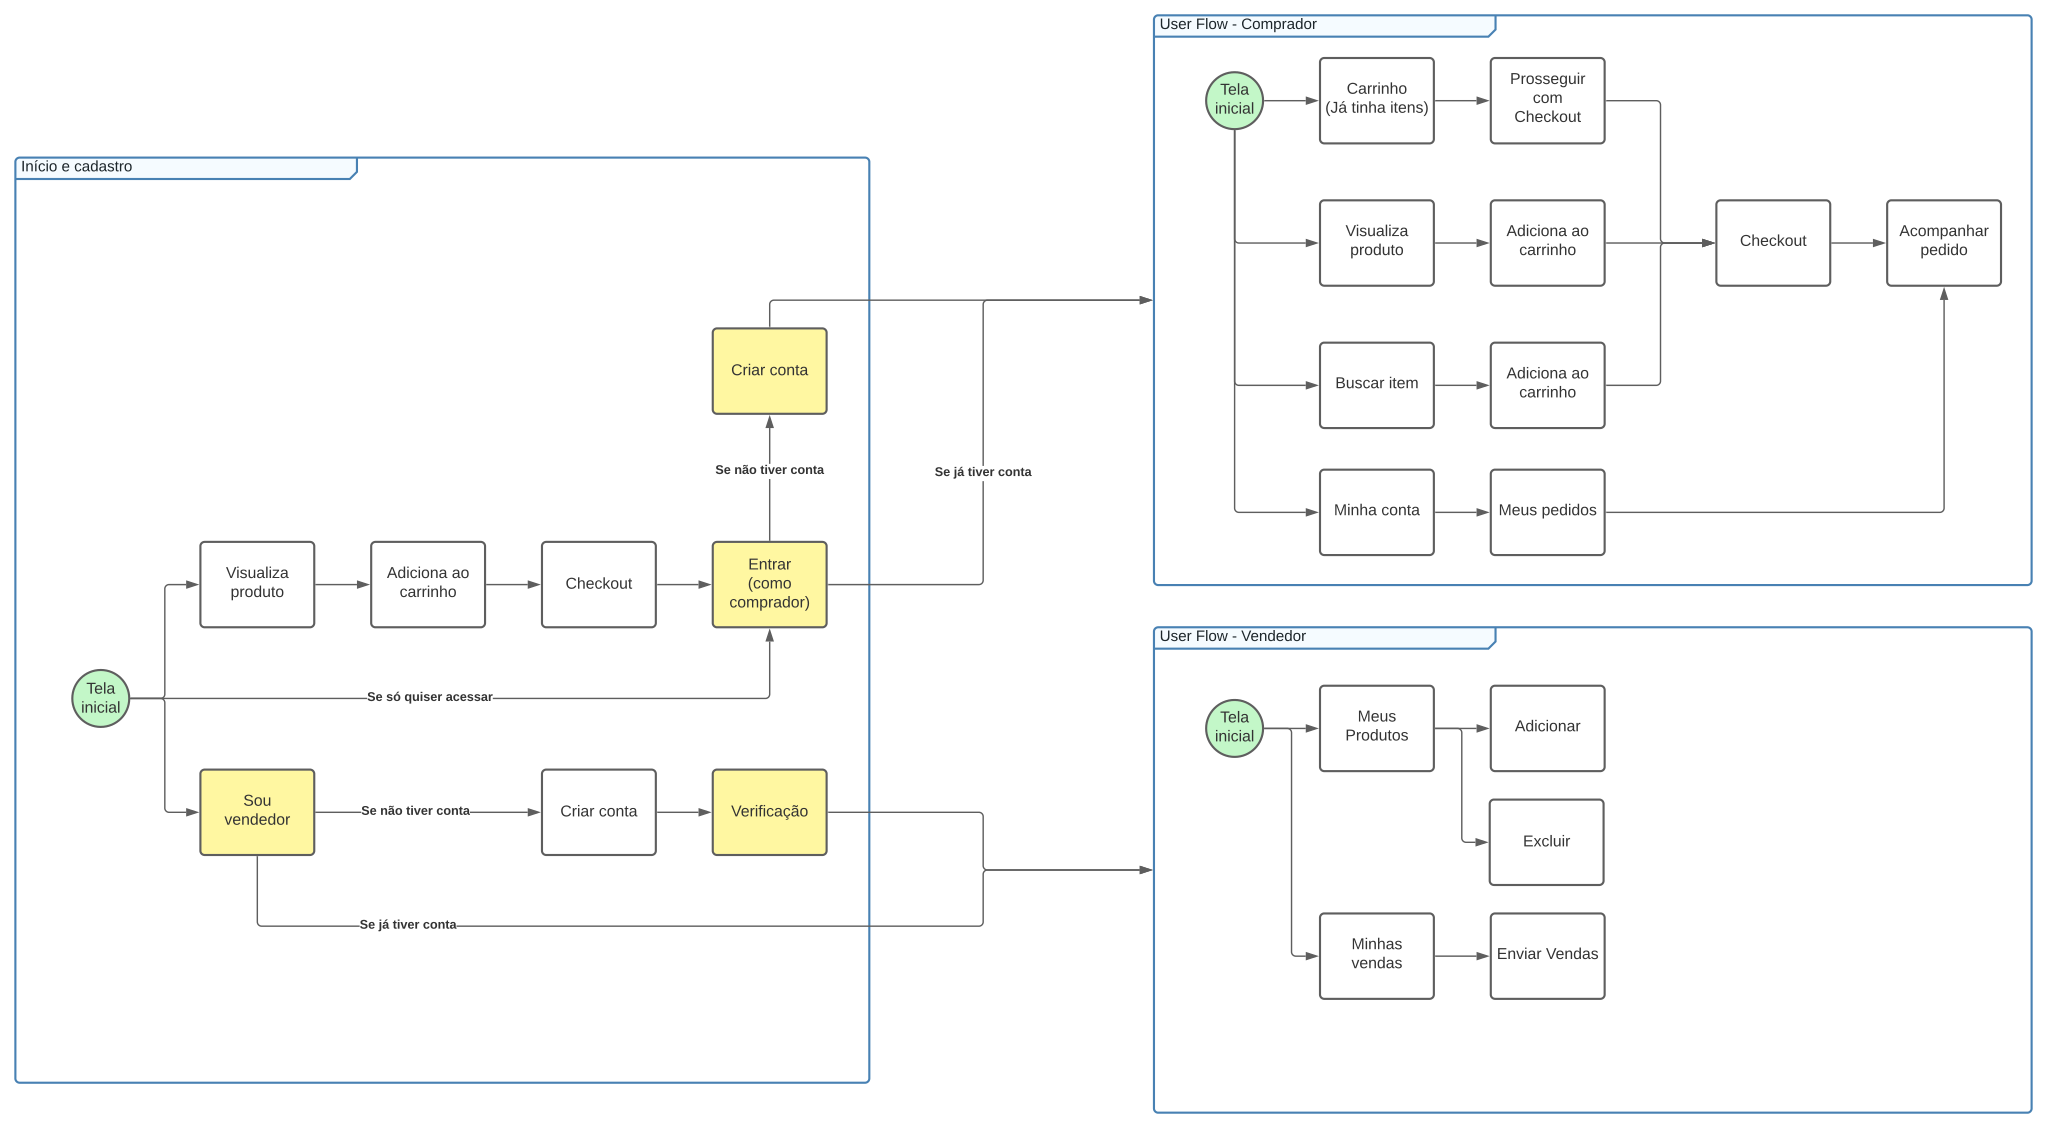
\includegraphics[width=0.6\textwidth]{img/User-Flow}
    \caption{Fluxo dos usuários "Comprador" e "Vendedor" (Desenvolvido pelos Autores).}
    \label{fig:diagrama-user-flow}
\end{figure}

Este diagrama oferece uma representação visual do percurso dos usuários, tanto "Comprador" quanto "Vendedor", dentro do protótipo. A análise detalhada desta representação é essencial para compreender as interações esperadas e identificar pontos cruciais de usabilidade. Dessa forma, estabelece-se uma base sólida para a próxima fase: a organização do código ASPX, onde traduziremos essa estrutura conceitual em implementação prática no Sistema de Marketplace.

O entendimento do fluxo do usuário é crucial para garantir uma experiência intuitiva e eficiente. Serão abordados aspectos como a navegação entre páginas, interações com elementos da interface, e feedbacks fornecidos ao usuário durante o processo de utilização.

Ao compreender o fluxo do usuário, estaremos preparados para a próxima etapa: a organização do código ASPX, onde transformaremos essa estrutura conceitual em uma implementação prática e funcional do Sistema de Marketplace.

\section{Estruturação do Código ASPX}

Na fase de desenvolvimento do Sistema de Marketplace, uma consideração crucial reside na estruturação eficaz do código ASPX, responsável por fornecer a interface gráfica através da plataforma ASP.net. A qualidade do código nessa etapa influencia diretamente a experiência do usuário e a eficiência operacional do sistema.

Nesta seção, exploraremos a organização do código ASPX, destacando princípios de design e as estratégias adotadas para garantir a coesão e a manutenibilidade do código. A compreensão detalhada dessa estrutura é fundamental para a transição suave da concepção do projeto para sua implementação prática.

\section{Visualização da Interface em Capturas de Tela}

\subsubsection{Carrinho}

\begin{figure}[htb]
    \centering
    \includegraphics[width=0.6\textwidth]{img/carrinho-desktop-print.jpg}
    \caption{Tela de Carrinho (Desenvolvido pelos Autores).}
    \label{fig:tela-de-carrinho-desktop}
\end{figure}

A tela do carrinho é o espaço virtual onde os usuários podem revisar e gerenciar os itens selecionados para compra. Nessa interface, eles podem adicionar, remover ou ajustar a quantidade de produtos no carrinho antes de prosseguir para o checkout.

\begin{lstlisting}[language=HTML, caption=Tela de Carrinho em ASPX, label=lst:aspx]

<%@ Page Title="Carrinho" Language="C#" MasterPageFile="~/Site.Master" AutoEventWireup="true" CodeBehind="Carrinho.aspx.cs" Inherits="UNIPPIMVIII.Carrinho" %>

<asp:Content ID="BodyContent" ContentPlaceHolderID="MainContent" runat="server">
    <h1>Carrinho</h1>
    <table class="table table-bordered">
        <thead>
            <tr class="bg-primary">
                <th scope="col"></th>
                <th scope="col">Produto</th>
                <th scope="col">Quantidade</th>
                <th scope="col">Preço unitário</th>
                <th scope="col">Preço total</th>
            </tr>
        </thead>
        <tbody>
            <tr>
                <th scope="row"><input type="checkbox" /></th>
                <td>Smartphone Nokia C21 ...</td>
                <td>1</td>
                <td>R$10,00</td>
                <td>R$10,00</td>
            </tr>            
        </tbody>
    </table>
    <br />
    <p>
        <a runat="server" href="~/Checkout.aspx"><button type="button" class="btn btn-primary" style="width:30%;height:auto;">Confirmar</button></a>
    </p>
</asp:Content>


\end{lstlisting}

\subsubsection{Checkout}

\begin{figure}[htb]
    \centering
    \includegraphics[width=0.6\textwidth]{img/checkout-desktop-print.jpg}
    \caption{Tela de Checkout (Desenvolvido pelos Autores).}
    \label{fig:tela-de-checkout-desktop}
\end{figure}


A tela de checkout é o ponto crucial onde os usuários finalizam suas compras. Aqui, eles fornecem informações de pagamento, endereço de entrega e revisam o resumo da compra antes de confirmar o pedido. Uma interface intuitiva é essencial para simplificar esse processo sensível.

\begin{lstlisting}[language=HTML, caption=Tela de Checkout em ASPX, label=lst:aspx]

<%@ Page Title="Checkout" Language="C#" MasterPageFile="~/Site.Master" AutoEventWireup="true" CodeBehind="Checkout.aspx.cs" Inherits="UNIPPIMVIII.Checkout" %>

<asp:Content ID="BodyContent" ContentPlaceHolderID="MainContent" runat="server">
    <h1>Checkout</h1>

    <p>Nome do remetente</p>
    <input type="text" />
    <p>CEP</p>
    <input type="text" />
    <p>Complemento</p>
    <input type="text" />
    <p>Número</p>
    <input type="text" />
    <p>Estado</p>
    <input type="text" />
    <p>Cidade</p>
    <input type="text" />
    <br />
    <p>
        <a runat="server" href="~/">
            <button type="button" class="btn btn-primary" style="width: 30%; height: auto;">Confirmar</button></a>
    </p>
</asp:Content>


\end{lstlisting}


\subsubsection{Login do Cliente}

\begin{figure}[htb]
    \centering
    \includegraphics[width=0.6\textwidth]{img/login-desktop-print.jpg}
    \caption{Tela de Login (Desenvolvido pelos Autores).}
    \label{fig:tela-de-login-desktop}
\end{figure}

A tela de login do cliente é a porta de entrada personalizada para usuários registrados. Aqui, eles inserem suas credenciais para acessar funcionalidades exclusivas, como histórico de compras, rastreamento de pedidos e configurações de conta.

\begin{lstlisting}[language=HTML, caption=Tela de Login em ASPX, label=lst:aspx]

<%@ Page Title="Login" Language="C#" MasterPageFile="~/Site.Master" AutoEventWireup="true" CodeBehind="LoginCliente.aspx.cs" Inherits="UNIPPIMVIII.LoginCliente" %>

<asp:Content ID="BodyContent" ContentPlaceHolderID="MainContent" runat="server">
    <div class="box-parent-login">
	<div class="well bg-white box-login">
		<h1 class="ls-login-logo"></h1>
		<form role="form">
			<fieldset>
 
				<div class="form-group ls-login-user">
					<label for="userLogin">Usuário</label>
					<input class="form-control ls-login-bg-user input-lg" id="userLogin" type="text" aria-label="Usuário" placeholder="Usuário">
				</div>
 
				<div class="form-group ls-login-password">
					<label for="userPassword">Senha</label>
					<input class="form-control ls-login-bg-password input-lg" id="userPassword" type="password" aria-label="Senha" placeholder="Senha">
				</div>
 
				<a href="#" class="ls-login-forgot">Esqueci minha senha</a>
 
				<input type="submit" value="Entrar" class="btn btn-primary btn-lg btn-block">
				<p class="txt-center ls-login-signup">Não possui um usuário na Locaweb?
					<a href="#">Cadastre-se agora</a>
				</p>
 
			</fieldset>
		</form>
	</div>
</div>
</asp:Content>

\end{lstlisting}

\subsubsection{Layout Principal}

\begin{figure}[htb]
    \centering
    \includegraphics[width=0.6\textwidth]{img/inicio-desktop-print.jpg}
    \caption{Tela de Início (Desenvolvido pelos Autores).}
    \label{fig:tela-de-inicio-desktop}
\end{figure}

O layout principal é a página inicial do Sistema de Marketplace, onde os usuários são recebidos com uma visão geral dos produtos em destaque, promoções e categorias. Essa tela desempenha um papel vital na navegação inicial e na exposição de produtos.

\begin{lstlisting}[language=HTML, caption=Tela Principal em ASPX, label=lst:aspx]

	<%@ Page Title="Pagina Inicial" Language="C#" MasterPageFile="~/Site.Master" AutoEventWireup="true" CodeBehind="Default.aspx.cs" Inherits="UNIPPIMVIII._Default" %>

	<asp:Content ID="BodyContent" ContentPlaceHolderID="MainContent" runat="server">
	
		<div class="row">
			<div class="col-md-5" style="margin:auto; display:flex">
				<img src="imgs/grupo_1830.png" />
			</div>
			<div class="col-md-7" style="height:311px;margin:auto;display:flex">
				<img src="imgs/grupo_1922.png"/>
			</div>
		</div>
		<br/>
		<br/>
		<br/>
		<div class="row">
			<h2>Roupas</h2>
		</div>
		<div class="row" >
			<div class="col-md-3">
				<a runat="server" href="~/Produto.aspx"><img src="imgs/roupa1.png" style="width:200px;height:200px;border:2px solid black"/></a>
			</div>
			<div class="col-md-3">
				<a runat="server" href="~/Produto.aspx"><img src="imgs/roupa2.png" style="width:200px;height:200px;border:2px solid black"/></a>
			</div>
			<div class="col-md-3">
				<a runat="server" href="~/Produto.aspx"><img src="imgs/roupa1.png" style="width:200px;height:200px;border:2px solid black"/></a>
			</div>
			<div class="col-md-3">
				<a runat="server" href="~/Produto.aspx"><img src="imgs/roupa2.png" style="width:200px;height:200px;border:2px solid black"/></a>
			</div>
		</div>
		<br />
		<br />
		<br />
		<div class="row">
			<h2>Celular</h2>
		</div>
		<div class="row" >
			<div class="col-md-3">
				<a runat="server" href="~/Produto.aspx"><img src="imgs/celular1.png" style="width:200px;height:200px;border:2px solid black"/></a>
			</div>
			<div class="col-md-3">
				<a runat="server" href="~/Produto.aspx"><img src="imgs/celular2.png" style="width:200px;height:200px;border:2px solid black"/></a>
			</div>
			<div class="col-md-3">
				<a runat="server" href="~/Produto.aspx"><img src="imgs/celular3.png" style="width:200px;height:200px;border:2px solid black"/></a>
			</div>
			<div class="col-md-3">
				<a runat="server" href="~/Produto.aspx"><img src="imgs/celular4.png" style="width:200px;height:200px;border:2px solid black"/></a>
			</div>
		</div>
	</asp:Content>
	

\end{lstlisting}

\subsubsection{Página de Produto}

\begin{figure}[htb]
    \centering
    \includegraphics[width=0.6\textwidth]{img/product-desktop-print.jpg}
    \caption{Tela de Produto (Desenvolvido pelos Autores).}
    \label{fig:tela-de-produto-desktop}
\end{figure}

Ao acessar a página de um produto específico, os usuários encontram detalhes abrangentes sobre o item, incluindo descrição, preço, avaliações e opções de compra. Uma interface clara e informativa é crucial para influenciar as decisões de compra nessa fase crítica.

\begin{lstlisting}[language=HTML, caption=Tela de Produto em ASPX, label=lst:aspx]

	<%@ Page Title="Produto" Language="C#" MasterPageFile="~/Site.Master" AutoEventWireup="true" CodeBehind="Produto.aspx.cs" Inherits="UNIPPIMVIII.Produto" %>

	<asp:Content ID="BodyContent" ContentPlaceHolderID="MainContent" runat="server">
		<div class="row">
			<div class="col-md-7">
				<h1>Smartphone Nokia c21 Plus 4g 128GB Tela HD+ 6,5 Câmera Dupla 13MP Android Bateria de 2 dias de duração +</h1>
				<h2>R$100,00</h2>
				<h3>Em até 12x sem juros</h3>
				<p>
				<a runat="server" href="Carrinho.aspx"><button type="button" class="btn btn-primary" style="margin:auto;width:70%;height:auto;">Adicionar ao Carrinho</button></a>
					</p>
				<br/>
				<a runat="server" href="Checkout.aspx"><button type="button" class="btn btn-light" style="margin:auto;width:70%;height:auto;">Comprar</button></a>
			</div>
			<div class="col-md-5">
				<img src="imgs/celular4.png" style="margin:auto;width:70%;height:auto;border:2px solid black" />
			</div>
		</div>
	</asp:Content>
	

\end{lstlisting}

\chapter{Tópicos Especiais de Programação Orientada a Objetos}\label{cap_topic_espec_de_progra}

\section{Estruturação do Código XML}

Com base na análise do fluxo do usuário para sistemas mobile, procedemos à criação do protótipo de baixa fidelidade utilizando o Android Studio como ambiente de desenvolvimento integrado (IDE), Kotlin como linguagem de programação e XML como linguagem de marcação.

Para otimizar a organização e manutenção do código, optamos por uma abordagem que divide as telas em arquivos XML distintos, proporcionando modularidade e clareza estrutural. Ao todo, foram desenvolvidas cinco telas, cada uma correspondendo a uma etapa específica do fluxo do usuário "Comprador".

\begin{figure}[htb]
    \centering
    \includegraphics[width=0.6\textwidth]{img/IDE-android-studio}
    \caption{IDE do Android Studio (Fonte: os Autores).}
    \label{fig:ide_android_studio}
\end{figure}

A estruturação modular permitiu uma implementação mais eficiente, facilitando a manutenção e aprimoramento de cada componente da interface. Cada tela foi cuidadosamente projetada e, posteriormente, vinculada aos seus respectivos arquivos em Kotlin, estabelecendo uma conexão fluida entre a lógica de programação e a apresentação visual.

Este enfoque na estruturação do código XML não apenas contribui para a coesão e clareza do código-fonte, mas também simplifica a implementação de futuras atualizações e a incorporação de novas funcionalidades ao Sistema de Marketplace para dispositivos móveis. Na próxima seção, exploraremos mais a fundo a integração desses elementos na programação Kotlin, detalhando como cada tela foi associada à lógica do aplicativo.

\section{Exibição da Interface em Capturas de Tela}

Nesta seção, apresentaremos capturas de tela que ilustram a interface do Sistema de Marketplace em sua fase de prototipagem para dispositivos móveis. Cada imagem corresponde a uma tela específica, proporcionando uma visão visual abrangente do design e da disposição dos elementos em diferentes etapas do processo.

\subsection{Tela: \texttt{carrinho.xml}}

\begin{figure}[htb]
    \centering
    \includegraphics[width=0.2\textwidth]{img/carrinho}
    \caption{Captura de Tela - Carrinho}
\end{figure}

A tela de carrinho exibe os produtos selecionados pelo usuário "Comprador", oferecendo uma visão consolidada das escolhas feitas durante a sessão de compras.

\begin{lstlisting}[language=XML, caption=Exemplo de Código XML, label=lst:xml]

<?xml version="1.0" encoding="utf-8"?>
<LinearLayout xmlns:android="http://schemas.android.com/apk/res/android"
    xmlns:app="http://schemas.android.com/apk/res-auto"
    xmlns:tools="http://schemas.android.com/tools"
    android:layout_width="match_parent"
    android:layout_height="match_parent"
    android:orientation="vertical">

    <!-- Header -->
    <RelativeLayout
        android:id="@+id/header"
        android:layout_width="match_parent"
        android:layout_height="wrap_content"
        android:background="#FFFFFF">

        <!-- Logotipo -->
        <ImageView
            android:id="@+id/logo"
            android:layout_width="80dp"
            android:layout_height="60dp"
            android:layout_centerVertical="true"
            android:layout_marginStart="25dp"
            android:layout_marginEnd="8dp"
            android:contentDescription="@string/logo"
            android:src="@drawable/logo" />

        <!-- Ícone de Perfil -->
        <ImageView
            android:id="@+id/menuIcon"
            android:layout_width="24dp"
            android:layout_height="24dp"
            android:layout_centerVertical="true"
            android:layout_marginEnd="15dp"
            android:layout_toStartOf="@id/profileIcon"
            android:contentDescription="@string/menu"
            android:src="@drawable/profile_icon" />

        <!-- Ícone de Menu -->
        <ImageView
            android:id="@+id/profileIcon"
            android:layout_width="24dp"
            android:layout_height="24dp"
            android:layout_alignParentEnd="true"
            android:layout_centerVertical="true"
            android:layout_marginEnd="25dp"
            android:contentDescription="@string/test"
            android:src="@drawable/menu_icon" />

    </RelativeLayout>

	<!-- Restante do código mandado em Anexo com esse documento -->

</LinearLayout>

\end{lstlisting}

\subsection{Tela: \texttt{checkout.xml}}

\begin{figure}[htb]
    \centering
    \includegraphics[width=0.2\textwidth]{img/checkout}
    \caption{Captura de Tela - Checkout}
\end{figure}

A tela de checkout apresenta o resumo da compra, permitindo ao usuário revisar os itens escolhidos, ajustar quantidades e proceder ao pagamento.

\begin{lstlisting}[language=XML, caption=Código XML da tela de Checkout, label=lst:xml]

	<?xml version="1.0" encoding="utf-8"?>
	<?xml version="1.0" encoding="utf-8"?>
	<LinearLayout xmlns:android="http://schemas.android.com/apk/res/android"
	
		android:layout_width="match_parent"
		android:layout_height="match_parent"
		android:orientation="vertical">
	
		<!-- Header -->
		<RelativeLayout
			android:id="@+id/header"
			android:layout_width="match_parent"
			android:layout_height="wrap_content"
			android:background="#FFFFFF">
	
			<!-- Logotipo -->
			<ImageView
				android:id="@+id/logo"
				android:layout_width="80dp"
				android:layout_height="60dp"
				android:layout_centerVertical="true"
				android:layout_marginStart="25dp"
				android:layout_marginEnd="8dp"
				android:contentDescription="@string/logo"
				android:src="@drawable/logo" />
	
			<!-- Ícone de Perfil -->
			<ImageView
				android:id="@+id/menuIcon"
				android:layout_width="24dp"
				android:layout_height="24dp"
				android:layout_centerVertical="true"
				android:layout_marginEnd="15dp"
				android:layout_toStartOf="@id/profileIcon"
				android:contentDescription="@string/menu"
				android:src="@drawable/profile_icon" />
	
			<!-- Ícone de Menu -->
			<ImageView
				android:id="@+id/profileIcon"
				android:layout_width="24dp"
				android:layout_height="24dp"
				android:layout_alignParentEnd="true"
				android:layout_centerVertical="true"
				android:layout_marginEnd="25dp"
				android:contentDescription="@string/test"
				android:src="@drawable/menu_icon" />
	
		</RelativeLayout>
		
		<!-- Restante do código mandado em Anexo com esse documento -->
	
	</LinearLayout>

\end{lstlisting}

\subsection{Tela: \texttt{logincliente.xml}}

\begin{figure}[htb]
    \centering
    \includegraphics[width=0.2\textwidth]{img/logincliente}
    \caption{Captura de Tela - Login do Cliente}
\end{figure}

A tela de login do cliente é o ponto de autenticação, onde o usuário pode acessar sua conta para personalizar a experiência de compra.

\begin{lstlisting}[language=XML, caption=Código da tela de Login, label=lst:xml]

	<?xml version="1.0" encoding="utf-8"?>
	<LinearLayout xmlns:android="http://schemas.android.com/apk/res/android"
		xmlns:app="http://schemas.android.com/apk/res-auto"
		xmlns:tools="http://schemas.android.com/tools"
		android:layout_width="match_parent"
		android:layout_height="match_parent"
		android:orientation="vertical">
	
		<!-- Header -->
		<RelativeLayout
			android:id="@+id/header"
			android:layout_width="match_parent"
			android:layout_height="wrap_content"
			android:background="#FFFFFF">
	
			<!-- Logotipo -->
			<ImageView
				android:id="@+id/logo"
				android:layout_width="80dp"
				android:layout_height="60dp"
				android:layout_centerVertical="true"
				android:layout_marginStart="25dp"
				android:layout_marginEnd="8dp"
				android:contentDescription="@string/logo"
				android:src="@drawable/logo" />
	
			<!-- Ícone de Perfil -->
			<ImageView
				android:id="@+id/menuIcon"
				android:layout_width="24dp"
				android:layout_height="24dp"
				android:layout_centerVertical="true"
				android:layout_marginEnd="15dp"
				android:layout_toStartOf="@id/profileIcon"
				android:contentDescription="@string/menu"
				android:src="@drawable/profile_icon" />
	
			<!-- Ícone de Menu -->
			<ImageView
				android:id="@+id/profileIcon"
				android:layout_width="24dp"
				android:layout_height="24dp"
				android:layout_alignParentEnd="true"
				android:layout_centerVertical="true"
				android:layout_marginEnd="25dp"
				android:contentDescription="@string/test"
				android:src="@drawable/menu_icon" />
	
		</RelativeLayout>
	
		<ScrollView
			android:layout_width="match_parent"
			android:layout_height="match_parent"
			android:background="#F1F0F3">
	
			<LinearLayout
				android:layout_width="match_parent"
				android:layout_height="wrap_content"
				android:orientation="vertical">
	
				<TextView
					android:layout_width="wrap_content"
					android:layout_height="wrap_content"
					android:layout_margin="100px"
					android:padding="8dp"
					android:text="Entrar"
					android:textColor="#91939F"
					android:textSize="20sp"
					android:textStyle="bold" />
	
					
			<!-- Restante do código mandado em Anexo com esse documento -->
	
	</LinearLayout>


\end{lstlisting}

\subsection{Tela: \texttt{main\_layout.xml}}

\begin{figure}[htb]
    \centering
    \includegraphics[width=0.2\textwidth]{img/main_layout}
    \caption{Captura de Tela - Layout Principal}
\end{figure}

A tela principal, ou \texttt{main\_layout.xml}, é a interface inicial do aplicativo, apresentando opções de navegação e categorias de produtos.

\begin{lstlisting}[language=XML, caption=ECódigo Layout Principal do portal, label=lst:xml]

	<?xml version="1.0" encoding="utf-8"?>
	<LinearLayout xmlns:android="http://schemas.android.com/apk/res/android"
		xmlns:app="http://schemas.android.com/apk/res-auto"
		xmlns:tools="http://schemas.android.com/tools"
		android:layout_width="match_parent"
		android:layout_height="match_parent"
		android:orientation="vertical">
	
		<!-- Header -->
		<RelativeLayout
			android:id="@+id/header"
			android:layout_width="match_parent"
			android:layout_height="wrap_content"
			android:background="#FFFFFF">
	
			<!-- Logotipo -->
			<ImageView
				android:id="@+id/logo"
				android:layout_width="80dp"
				android:layout_height="60dp"
				android:layout_centerVertical="true"
				android:layout_marginStart="25dp"
				android:layout_marginEnd="8dp"
				android:contentDescription="@string/logo"
				android:src="@drawable/logo" />
	
			<!-- Ícone de Perfil -->
			<ImageView
				android:id="@+id/menuIcon"
				android:layout_width="24dp"
				android:layout_height="24dp"
				android:layout_centerVertical="true"
				android:layout_marginEnd="15dp"
				android:layout_toStartOf="@id/profileIcon"
				android:contentDescription="@string/menu"
				android:src="@drawable/profile_icon" />
	
			<!-- Ícone de Menu -->
			<ImageView
				android:id="@+id/profileIcon"
				android:layout_width="24dp"
				android:layout_height="24dp"
				android:layout_alignParentEnd="true"
				android:layout_centerVertical="true"
				android:layout_marginEnd="25dp"
				android:contentDescription="@string/test"
				android:src="@drawable/menu_icon" />
	
		</RelativeLayout>
	
	
		<!-- Restante do código mandado em Anexo com esse documento -->
	
	</LinearLayout>

\end{lstlisting}

\subsection{Tela: \texttt{product.xml}}

\begin{figure}[htb]
    \centering
    \includegraphics[width=0.2\textwidth]{img/product}
    \caption{Captura de Tela - Detalhes do Produto}
\end{figure}

A tela de detalhes do produto exibe informações específicas sobre um item selecionado, proporcionando ao usuário uma visão mais aprofundada antes da compra.

\begin{lstlisting}[language=XML, caption=Exemplo de Código XML, label=lst:xml]

	<?xml version="1.0" encoding="utf-8"?>
	<LinearLayout xmlns:android="http://schemas.android.com/apk/res/android"
		xmlns:app="http://schemas.android.com/apk/res-auto"
		xmlns:tools="http://schemas.android.com/tools"
		android:layout_width="match_parent"
		android:layout_height="match_parent"
		android:orientation="vertical">
	
		<!-- Header -->
		<RelativeLayout
			android:id="@+id/header"
			android:layout_width="match_parent"
			android:layout_height="wrap_content"
			android:background="#FFFFFF">
	
			<!-- Logotipo -->
			<ImageView
				android:id="@+id/logo"
				android:layout_width="80dp"
				android:layout_height="60dp"
				android:layout_centerVertical="true"
				android:layout_marginStart="25dp"
				android:layout_marginEnd="8dp"
				android:contentDescription="@string/logo"
				android:src="@drawable/logo" />
	
			<!-- Ícone de Perfil -->
			<ImageView
				android:id="@+id/menuIcon"
				android:layout_width="24dp"
				android:layout_height="24dp"
				android:layout_centerVertical="true"
				android:layout_marginEnd="15dp"
				android:layout_toStartOf="@id/profileIcon"
				android:contentDescription="@string/menu"
				android:src="@drawable/profile_icon" />
	
			<!-- Ícone de Menu -->
			<ImageView
				android:id="@+id/profileIcon"
				android:layout_width="24dp"
				android:layout_height="24dp"
				android:layout_alignParentEnd="true"
				android:layout_centerVertical="true"
				android:layout_marginEnd="25dp"
				android:contentDescription="@string/test"
				android:src="@drawable/menu_icon" />
	
		</RelativeLayout>
	
		<ScrollView
			android:layout_width="match_parent"
			android:layout_height="match_parent"
			android:background="#FCFBFF">
	
			<LinearLayout
				android:layout_width="match_parent"
				android:layout_height="wrap_content"
				android:orientation="vertical">
	
				<TextView
					android:layout_margin="100px"
					android:layout_width="wrap_content"
					android:layout_height="wrap_content"
					android:text="Smartphone Nokia C21 Plus 4G 128GB Tela HD+ 6,5 Câm Dupla 13MP Android Bateria de 2 dias de duração +"
					android:textColor="#91939F"
					android:textSize="20sp"
					android:textStyle="bold"
					android:padding="8dp"/>
	
				<androidx.cardview.widget.CardView
					android:layout_width="match_parent"
					android:layout_height="wrap_content"
					android:layout_margin="16dp"
					android:cardBackgroundColor="#ffffff"
					android:layout_gravity="center"
					android:radius="16dp">
	
		<!-- Restante do código mandado em Anexo com esse documento -->
	
	</LinearLayout>

\end{lstlisting}

Essas capturas de tela oferecem uma representação visual do cuidadoso design da interface do usuário, facilitando a compreensão da experiência que o Sistema de Marketplace busca proporcionar aos usuários móveis.

\chapter{Programação Orientada a Objetos II}\label{cap_program_orientada_a_objetos}

O capítulo de Programação Orientada a Objetos II concentra-se em aspectos fundamentais para o desenvolvimento eficiente do Sistema de Marketplace proposto. Abordaremos a modelagem de entidades e relacionamentos no banco de dados, a estruturação do código em C\# para acesso às classes e entidades, além da implementação crucial da classe repositório 'CarrinhoRepository'.

\subsection{Modelagem de Entidades e Relacionamentos no Banco de Dados}

Antes de adentrar a implementação em código, é imperativo estabelecer uma sólida modelagem de entidades e seus relacionamentos no banco de dados. Este passo é crucial para a integridade e eficiência do sistema. A definição clara das entidades, como Cliente, Carrinho, Produto e Vendedor, juntamente com seus relacionamentos, moldará a estrutura do banco de dados e, por consequência, a dinâmica do Sistema de Marketplace.

\begin{lstlisting}[language={[Sharp]C}, caption=Entidades do código C\#, label=lst:entidades]
	using System ; 
	using System.Collections.Generic;  
	using System.Linq;
	using System.Text;  
	using System.Threading.Task s;
	
	public class Cliente
	{
		public int Id { get; set; }
		public string Nome { get; set; }
		public string Cpf { get; set; }
		public string Email { get; set; }
		public string Senha { get; set; }
		public string Endereco { get; set; }
	
		public Carrinho Carrinho { get; set; }
	}
	
	public class Carrinho
	{
		public int Id { get; set; }
		public DateTime DataPedido { get; set; }
		public decimal ValorTotal { get; set; }
		public string StatusPedido { get; set; }
	
		public Cliente Cliente { get; set; }
		public List<Produto> Produtos { get; set; }
	}
	
	public class Produto
	{
		public int Id { get; set; }
		public string Descricao { get; set; }
		public decimal Preco { get; set; }
		public string Imagem { get; set; }
		public string Status { get; set; }
	
		public Vendedor Vendedor { get; set; }
		public Categoria Categoria { get; set; }
	}
	
	public class Vendedor
	{
			public int Id { get; set; }
			public string RazaoSocial { get; set; }
			public string NomeFantasia { get; set; }
			public string Cnpj { get; set; }
			public string Email { get; set; }
			public string Senha { get; set; }
			public string Endereco { get; set; }
			public decimal Comissao { get; set; }
	}
\end{lstlisting}

Para representar a conexão das diversas Entidades com o Banco de Dados também desenvolvemos um código C\# presente no seuguinte trecho:


\begin{lstlisting}[language={[Sharp]C}, caption=Conexão com a Data Base, label=lst:conexao]
using Microsoft.EntityFrameworkCore;

public class LojaContext : DbContext
	{
		public DbSet<Cliente> Clientes { get; set; }
		public DbSet<Carrinho> Carrinhos { get; set; }
		public DbSet<Produto> Produtos { get; set; }
		public DbSet<Vendedor> Vendedores { get; set; }
		public DbSet<Categoria> Categorias { get; set; }

		protected override void OnConfiguring(DbContextOptionsBuilder optionsBuilder)
		{
			optionsBuilder.UseSqlServer("Data Source=(localdb)\\MSSQLLocalDB;Initial Catalog=LojaDB;Integrated Security=True");
		}
	}
\end{lstlisting}

\subsection{Estruturação do Código \texttt{C\#} para Acesso às Classes e Entidades}

Com a modelagem de dados consolidada, avançaremos para a estruturação do código em C\#. Este tópico abordará a forma como as classes e entidades definidas anteriormente serão acessadas e manipuladas no ambiente do Sistema de Marketplace. A clareza e eficácia dessa estruturação são cruciais para garantir a coerência entre a representação do modelo no código e no banco de dados.

\subsection{Implementação da Classe Repositório 'CarrinhoRepository'}

A implementação da classe 'CarrinhoRepository' desempenha um papel central na gestão dos carrinhos de compras. Essa classe é responsável por operações como adicionar itens, remover produtos, calcular o total da compra e outras ações relacionadas ao carrinho do cliente. A eficiência e correção dessa implementação influenciam diretamente a experiência do usuário ao utilizar o Sistema de Marketplace.

No decorrer deste capítulo, cada tópico será explorado detalhadamente, proporcionando uma compreensão abrangente da Programação Orientada a Objetos II no contexto do desenvolvimento do Sistema de Marketplace. O objetivo é não apenas implementar funcionalidades, mas também assegurar a manutenibilidade e escalabilidade do sistema ao longo do tempo.

\begin{lstlisting}[language={[Sharp]C}, caption=DataBase, label=lst:basedata]
public class CarrinhoRepository
{
    private readonly LojaContext _context;

    public CarrinhoRepository(LojaContext context)
    {
        _context = context;
    }

    public async Task AdicionarCarrinhoAsync(Carrinho carrinho)
    {
        await _context.Carrinhos.AddAsync(carrinho);
        await _context.SaveChangesAsync();
    }

    public async Task AtualizarCarrinhoAsync(Carrinho carrinho)
    {
        _context.Entry(carrinho).State = EntityState.Modified;
        await _context.SaveChangesAsync();
    }

    public async Task ExcluirCarrinhoAsync(Carrinho carrinho)
    {
        _context.Carrinhos.Remove(carrinho);
        await _context.SaveChangesAsync();
    }

    public async Task<Carrinho> ObterPorIdAsync(int id)
    {
        return await _context.Carrinhos.FindAsync(id);
    }

    public async Task<List<Carrinho>> ObterTodosAsync()
    {
        return await _context.Carrinhos.ToListAsync();
	}
}
\end{lstlisting}

\chapter{Conclusão}\label{cap_conclusao}

O desenvolvimento acelerado da tecnologia continua a transformar de maneira expressiva o panorama comercial, guiando a transição para plataformas digitais que simplificam e agilizam as transações comerciais. Em resposta a esse cenário dinâmico, o Projeto Integrado Multidisciplinar (PIM) propôs e delineou a concepção e implementação de um Sistema de Marketplace, oferecendo uma abordagem abrangente para a compra e venda de uma extensa gama de produtos, acessível tanto por aplicativos móveis quanto por navegadores web.

O cerne deste projeto reside na convergência de disciplinas cruciais, com destaque para Desenvolvimento de Software para Internet, Tópicos Especiais de Programação Orientada a Objetos e Programação Orientada a Objetos II. No âmbito do Desenvolvimento de Software para Internet, a exploração dos códigos ASPX para a criação da interface gráfica usando ASP.net foi detalhada, com documentação por meio de capturas de tela e inclusão direta do código ASPX neste trabalho.

Na esfera dos Tópicos Especiais de Programação Orientada a Objetos, este trabalho apresentou um protótipo de interface gráfica para dispositivos Android, desenvolvido em XML. As capturas de tela e o código XML integrados ao documento oferecem uma visão holística do desenvolvimento orientado a objetos voltado para interfaces móveis.

A Programação Orientada a Objetos II foi abordada de maneira abrangente, com a implementação do código \texttt{C\#} responsável pelo acesso ao Banco de Dados. As classes de entidades fundamentais para o sistema - Cliente, Carrinho, Produto e Vendedor - foram codificadas de maneira apropriada. A classe CarrinhoRepository, crucial na gestão dos carrinhos de compras, foi desenvolvida com seus métodos implementados, assegurando a eficiência funcional do Sistema de Marketplace.

Este trabalho, além de apresentar uma proposta inovadora de Sistema de Marketplace, destaca a aplicação prática dos conhecimentos adquiridos ao longo das disciplinas. A solução tecnológica resultante é robusta e alinhada com as exigências contemporâneas do comércio digital. Ao integrar teoria e prática, este projeto não apenas representa uma conquista acadêmica, mas também ressalta a relevância e a aplicabilidade dos conceitos explorados.

Os autores, ao concluírem este projeto, reafirmam o compromisso com a excelência acadêmica e com a busca contínua por soluções inovadoras no campo da tecnologia. Este Sistema de Marketplace não é apenas o resultado de esforços acadêmicos, mas uma contribuição tangível para a evolução do cenário comercial digital.

\begin{thebibliography}{99}
    
\bibitem{robsoncamargo}
    ROBSON CAMARGO. PMBOK: O que é e qual sua importância no gerenciamento de projetos? Disponível em: \url{https://robsoncamargo.com.br/blog/PMBOK}. Acesso em 2023.

\bibitem{totvs}
    TOTVS. O que é PMBOK e como ele auxilia no gerenciamento de projetos? Disponível em: \url{https://www.totvs.com/blog/negocios/pmbok/}. Acesso em 2023.

\bibitem{blogaevo}
    AEVO. PMBOK: Guia completo para entender tudo sobre a metodologia! Disponível em: \url{https://blog.aevo.com.br/pmbok-guia-completo/}. Acesso em 2023.

\end{thebibliography}

%---------------------------------------------------------------------
% INDICE REMISSIVO
%---------------------------------------------------------------------
\phantompart
\printindex
%---------------------------------------------------------------------

\end{document}
